\section{Introduction}

In the previous chapter, we have focused on compressible active nematic gels pertinent to the sparse actin cytoskeleton, in which the mechanism of density patterning by self-reinforcing flows couples to nematic ordering. In such models,  the nematic order parameter can can vary between 0 and 1 and hence nematic order defects are not topological requirements. Other active nematic systems with high-density and/or long filaments, such as microtubule-kinesin gels, exhibit high local order everywhere except at defects, which are motile and dominate the dynamics  \cite{ndlec1997, surrey2001,sanchez2012}. Such systems are  well described by  active nematic liquid crystal (LC) theories, which commonly disregard density effects and where susceptibility parameters favor high local order \cite{zhang2018,kumar2018}. When confined to a deformable surface, liquid-crystalline systems develop orientational defects which strongly interact with local curvature, as shown in active and passive vesicles \cite{keber2014,xing2012} and during hydra morphogenesis \cite{maroudas2021}. Activity can modify the nature of defects and also induce complex dynamical states involving shape and defect reconfigurations and persistent interfacial flows. In active nematic vesicles, the bilayer where the nematic gel is confined imposes local inextensibility of the flow and provides bending resistance. 

Inextensibe active LC deformable surfaces  fall within the theoretical framework developed in Chapter~\ref{chap_7}. As discussed in the introduction of Part II of this thesis, Chapter~\ref{chap_6}, the general computational treatment of such models is challenging with only a handful of references addressing the coupled dynamics of defects and shape. To describe interfacial field theories on curved and time-evolving interfaces, there are two broad  approaches, one expressing the theories in  curvilinear coordinates adapted to the surface, and another one expressing them in Cartesian coordinates of ambient space and then projecting them on the surface. The curvilinear approach requires the language of differential geometry whereas the mathematical formulation and implementation of the Cartesian approach is simpler. However, the Cartesian approach is less efficient in that tangential fields are represented as 3D fields along with constraints. Here, we follow the curvilinear approach. To take advantage computationally of the mathematical efficiency of the curvilinear approach, one needs to approximate numerically tangent vector and tensor fields on a surface, which is not trivial because both the components and the basis vectors depend on position. Other computational challenges include the need of a smooth numerical representation of the surface, e.g.~to compute square integrable curvatures, handling large deformations and mesh distortions, or the requirement of an inf-sup compatible discretization of the Lagrange multiplier fields imposing local inextensibility. 

The rest of the Chapter is organized as follows. Section~\ref{chap8sec1}  describes the theoretical model for an active inextensible nematic fluid vesicle.  In Section~\ref{chap8sec2}, we propose a computational framework involving an efficient numerical solution of the governing equations discretized in space and time. Section~\ref{chap8sec3} explores computationally the tight interplay between dynamics of defects and curvature, first for passive vesicles with different geometric properties and then for active nematic vesicles. %In Section~\ref{chap8sec4}, we summarize our findings, outline the limitations of our approach and propose avenues for future research. 


\section{Governing equations based on Onsager's formalism}\label{chap8sec1}

We consider a thin and inextensible active nematic layer, whose shape is described by a time-evolving surface $A$ parametrized as described in Chapter~\ref{chap_7}, and whose orientational order is described by a tangential nematic tensor field, Eq.~(\ref{27_II}). The three-dimensional velocity field with tangential $\bm{v}$ and normal components $v_{N}$, i.e.~$\bm{V} = \bm{v} + v_{N}\bm{N}$, describes the interfacial flows and the rate-of-change of shape, whereas the Jaumann derivative  of the nematic tensor, $\widehat{\bm{q}}$, characterizes changes in nematic order. To impose local inextensibility, we resort to a Lagrange multiplier tension-like field $T$, whereas we enforce conservation of enclosed volume with a Lagrange multiplier pressure difference $P$.


%We characterize the rate of change of $\bm{q}$ with the Jaumann derivative $\widehat{\bm{q}}$ given by which measures the rate of change of the components of $\bm{q}$  viewed by an observer that flows and rotates with $\bm{v}$; thus, $\widehat{\bm{q}}$ is zero if $\bm{q}$ is advected and rotated by the flow without any further rearrangements of the nematic field. For a surface that is inextensible under both tension and compression. This constraint would have to be expressed by an isotropic tension field $T$. Lastly, we use pressure field $P$ to enforce the conservation of global volume due to osmotic effects.


We derive the governing equations of an active nematic system at low Reynolds numbers following non-linear Onsager's variational formalism. In this formalism, one needs to identify the free-energy of the system, $\mathcal{F}$, and the dissipation and power potentials, $\mathcal{D}$ and $\mathcal{P}$. 
The governing equations are obtained by minimizing the Rayleighian $\mathcal{R}=\dot{\mathcal{F}}+\mathcal{D}+\mathcal{P}$, where $\dot{\mathcal{F}}$ is the rate of change of the free energy.  The elastic behavior of the vesicle surface $\mathcal{F}$ is given by
\begin{equation} \label{9_1}
   \mathcal{F}[\bm{q}, \bm{x}] =\underset{A}{\int} \left(\frac{ \mathcal{B} }{2} H^{2} - \frac{a}{2}S^{2} + \frac{b}{8} S^{4} + \frac{L}{2}\nabla_c q_{ab} \nabla^c q^{ab} \right) \,d A \, ,
\end{equation}
where $H = g^{ab}k_{ab}$ is the local mean curvature. The first term above is the Helfrich bending energy of the membrane.  The second and third terms favor spontaneous nematic ordering on the membrane order parameter $S_0 = \sqrt{2a/b}$, where $a$ and $b$ are positive material constants. The last term is the Frank energy, controlled by the Frank constant $L$. Above the nematic correlation length $\ell_q = \sqrt{L/(2a)}$, the second and third terms dominates over the Frank term.

The dissipation potential is given by 
\begin{align}  \label{9_2}
    \mathcal{D}[\bm{q}, \bm{x};  \bm{V}, \widehat{\bm{q}}]   = \underset{A}{\int} \left[  \eta  d_{ab} d^{ab}+   \frac{\eta_{\text{rot}}}{2}  \widehat{q}_{ab}\widehat{q}^{ab} +\beta  d_{ab} \widehat{q}^{ab}   +  \frac{\gamma}{2} \left(v_a v^a + v_N^2\right) \right]   dA , \end{align}
where the first term is the shear dissipation potential, with $\eta$ the 2D membrane viscosity, the second term is the nematic dissipation potential, the term third captures the dissipative coupling between shear rate and changed in nematic order, and the last term models the frictional drag of the bilayer with its environments.

The power supply to the system by activity is characterized by the power potential
 \begin{align}  \label{9_3}
  \mathcal{P} \left[\bm{q}, \bm{x};  \bm{V} \right]  &=\underset{A}{\int} \lambda_{\rm ansio}q^{ab}d_{ab} dA,
 \end{align}
where $\lambda_{\rm aniso}>0$ for a contractile system and   $\lambda_{\rm aniso}<0$ for an extensile system such as microtubule-kinesin gels. We impose the inextensibility  and volume conservation using the constraint potential \begin{equation} \label{9_4}
    \mathcal{Q}\left[\bm{x};\bm{V}, T,P \right] = \underset{A}{\int}  T d^{a}_{\,a}     d A +  P \underset{A}{\int}  v_N  d A,
\end{equation}
To form the Lagrangian of the system, we need to compute the rate of change of the free-energy in Eq.~(\ref{9_1}). Because the surface is inextensible, the local changes in area and density are zero and we have the simple expression  $\mathcal{\dot{F}} =\underset{A}{\int} \mathcal{L}_{\bm{V}} f dA$.

We emphasize that these functionals intimately couple tangential flows in the fluid membrane, given by $\bm{v}$, and shape changes, given by $v_N$. Indeed, the rate-of-deformation tensor $\bm{d}$ involves these two velocities, see Eq.~(\ref{eq6:d}), and this tensor appears in each of the functionals involved in the system Lagrangian both explicitly and through the Jaumann derivative of the nematic tensor.

Particularizing the generic Euler-Lagrange equations obtained in Chapter~\ref{chap_7} to the present model, the governing equations are summarized in  Box~D. 


\begin{center}
\begin{mybox}{gray}{\center{\textbf{Box~D: Governing equations for an inextensible active nematic liquid crystalline membrane}}}
		
		\textbf{Generalized force balance for nematic field}
		\begin{equation}  \label{box_d_eq_1}
			\eta_{\text{rot}} \widehat{q}^{ab} +( 2a+bS^2 ) q^{ab} -  L\Delta q^{ab}   +\beta  d^{\textup{dev} \, ab}   = 0.
		\end{equation}
		
		\textbf{In-plane balance of linear momentum}:
		\begin{equation} \label{box_d_eq_2}
			\nabla_b \left(\sigma^{\textup{s} \, ab} + \sigma^{\textup{a} \, ab }   \right) -\sigma_N^b k^a_{~ b}= \gamma  v^a.
		\end{equation}
		
		\textbf{Out-of-plane  balance of linear momentum}:
		\begin{equation} \label{box_d_eq_3}
			\nabla_a \sigma^a_N - \sigma^{\textup{s}  \, ab} k_{ab} - \gamma v_N  + P = 0.
		\end{equation}
		
		\textbf{Constitutive relations}:
		\newline
		Power-conjugate to the rate-of-deformation tensor $d_{ab}$:
		\begin{align} \label{box_d_eq_4}
			\sigma^{\textup{s} \, ab}  =    2\eta d^{ab} -\mathcal{B}Hk^{ab}  -L\nabla^a q_{cd} \nabla^b q^{cd}    + \beta \widehat{q}^{ab}   +  \lambda_{\rm aniso} q^{ab}  . 
		\end{align}
		Power-conjugate to the in-plane and out-of-plane spins:
		\begin{align}  \label{box_d_eq_5}
			\sigma^{\textup{a} \, cd } = \frac{1}{2}\left(m^{ab} k_{ab} - \nabla_a m_N^a\right)\epsilon^{cd},
			\;\;\;\;\;\;\;\;
			\sigma_{N}^a  =- \epsilon^a_{~b} m_N^{c} k^{~b}_{c} - \epsilon^a_{~b}\nabla_c m^{cb}.
		\end{align}
		Power-conjugate to the gradients of the spins
		\begin{equation}  \label{box_d_eq_6}
			m_{N}^c= 2 L \epsilon_{fg} \nabla^c q^{af} q^g_{~a},
			\;\;\;\;\;\;\;\; m^{ab} = - \mathcal{B} Hg^{ab}.
		\end{equation}
		
		\textbf{Constraints}
		
		Incompressibility constraint:
		\begin{equation}  \label{box_d_eq_7}
			d^a_{~a} = 0.
		\end{equation}
		Balance of enclosed (incompressible) fluid:
		\begin{equation}  \label{box_d_eq_8}
			{\int_A}  v_N d A = 0.
		\end{equation}
	\end{mybox} \label{Box3}
\end{center}



\section{Numerical discretization} \label{chap8sec2}

 In this Section, we propose a method to discretize the governing equations in space and time. As in the previous chapter, we discretize spatial fields using finite elements and time using finite differences, and we derive the discrete equations from a time-discrete incremental Onsager principle, which grants nonlinear stability. One important decision when describing interfacial problems on fluid membranes is whether the parametrization follows material particles (Lagrangian parametrization) or not. A strictly Eulerian approach, such as that considered in the 2D model of Chapter \ref{chap_3}, is not meaningful for a deforming surface since surface motion is necessarily Lagrangian, but arbitrarily Lagrangian-Eulerian approaches are possible \cite{torres2019}. Here, we adopt a Lagrangian approach, which is mathematically and conceptually simple but requires remeshing algorithms to avoid excessive element distortion as a result of interfacial flows. 
 
 Space discretization of the present theory is challenging in various ways. First, because our theory involves surface curvature and Christoffel symbols, the numerical parametrization of the surface needs to be smooth, at least $C^1$ with continuous first derivatives. We consider Loop subdivision finite elements defined over triangulated surfaces. This method is an extension of splines to unstructured triangular grids, and leads to  smooth numerical surfaces. Second, we  need to choose a finite element space for the Lagrange multiplier field $T$ compatible with that of velocities. We address this by resorting to a macro-element approach adapted to subdivision approximations.  Third, we need to develop an efficient approximation for the traceless and symmetric tangential nematic field over a curved surface.  
 
 \subsection{Space discretization}

%We note that our model involves functionals that depend on curvature tensors and Christoffel  symbols. As a result, they contain second-order derivatives of fields and hence the finite-element solution requires $C^1$ interpolation. In particular, to ensure the energy is finite, the shape functions, as well as their first and second derivatives, should be square-integrable. For this reason, we use a higher-order Loop subdivision basis function on triangulated surfaces, guaranteed to be $C^2$ continuous everywhere except in the vicinity of irregular points where they are $C^1$ continuous. At the highest level of description, we may say that subdivision schemes construct smooth surfaces through a limiting procedure of repeated refinement starting from an initial mesh. This initial mesh will also be referred to as the control mesh of the surface. Generally, subdivision schemes consist of two steps. First, the mesh is refined, e.g., all faces are quadrisected, followed by the computation of new nodal positions. These positions are simple, linear functions of the nodal positions of the coarser mesh. These computations are local,i.e., they involve only nodal positions of the coarser mesh within a small, finite topological neighborhood, leading to very efficient implementations. Using a suitable choice of weights, such subdivision schemes can be designed to produce a smooth surface in the limit. Subdivision methods which result in limit surfaces whose curvature tensor is square-integrable are especially appealing for geometrical modeling applications and for thin-shell analysis.

\subsubsection*{Numerical approximation of kinematics}

Subdivision surfaces is a technology originally developed in computer graphics to numerically represent smooth surfaces, which was later adapted to the finite element context to solve thin shell and other interfacial partial differential equations  \cite{loop1987,stam1998,cirak2000,cirak2011,torres2019}. The discrete surface is represented by a surface triangulation, called control mesh, with $E= 1,....,N_e$ triangular elements and $I= 1,....,N_n$ nodes or vertices with position vector $\bm{x}_I\in\mathbb{R}^3$. The vertices are called control points. The method provides a prescription to define time-dependent element-wise local parametrizations of the form
\begin{equation} \label{9_17}
    \bm{x}= \bm{\phi}^E(\bm{\xi},t)= \underset{I \in R^E}{\mathrm{\sum}} B_I(\bm{\xi})\bm{x}_I(t),
\end{equation} 
where $R^E$ denotes the set of nodes belonging to element $E$ and to the first ring of elements adjacent to element $E$,  $B_I$ are the Loop subdivision basis functions defined over a reference triangular domain with coordinates $\bm{\xi} = (\xi^1, \xi^2)$, and $\bm{x}_I(t) = x^A_I(t) \bm{i}_A$ is the time-dependent position of vertex $I$ expressed in a Cartesian basis of $\mathbb{R}^3$. See Fig.~\ref{fig_1}(a) for an illustration. A vertex on the mesh is said to be regular if it is connected to exactly six other vertices on the triangulation. If all nodes of element $E$ are regular, then $B_I$ are explicitly known cubic box splines. Otherwise, their calculation is more involved.   

At any given time, the image of the reference triangular domain by the local chart $\bm{\phi}^E(\bm{\xi},t)$ is a curved triangle, which we denote by $A^E$. The subdivision method guarantees that these curved triangles do not overlap and that their union  $A = \bigcup_{E=1}^{N_e} A^E$ is regular surface, $C^2$ continuous everywhere except at irregular points where it is $C^1$.


\begin{figure}
	\centering
	\hspace*{-0.5cm}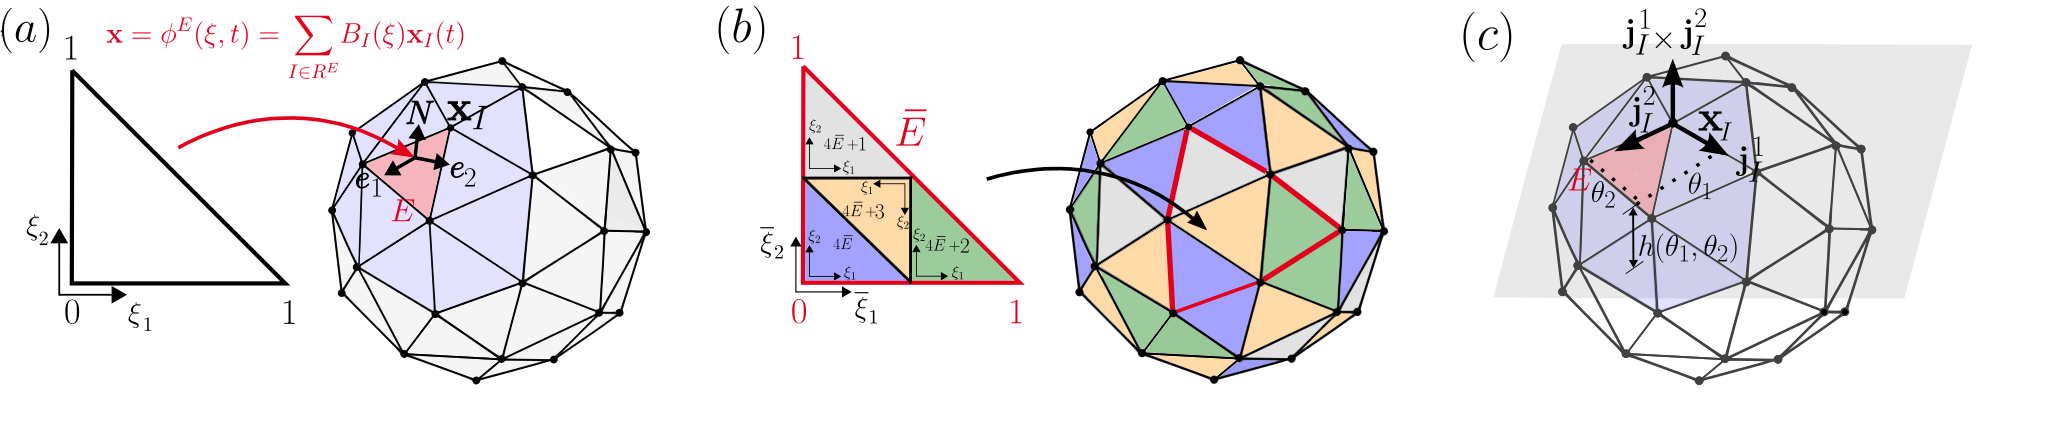
\includegraphics[width=1.\textwidth]{fig_sec_2_chap_4_1_1.pdf}
	\caption{\textbf{Illustration of space discretization.}  (a) Element-wise parametrization of the surface, $\bm{\phi}^E(\xi^1, \xi^2, t)$, using subdivision basis functions from a fixed reference domain. This local parametrization on a given element (shaded in red) depends on the nodes belonging to the one-ring of elements surrounding it (shaded un blue). (b) Nested meshes required to construct an inf-sup compatible discretization. Positions and velocities are approximated on the fine mesh, whereas the Lagrange multiplier field $T$ imposing local inextensibility is approximated on the coarse mesh. The figure also illustrates the correspondence between the reference coordinates of coarse and refine elements. (c) A local Monge parametrization of the surface, $\bm{\varphi}^I(\bm{\theta})$, is defined around each vertex $I$ in the mesh in terms of the height of a point in the surface $h(\bm{\theta})$ relative to a plane tangent to the surface at that vertex. This parametrization is expressed in terms of Cartesian coordinates of the plane $(\theta^1, \theta^2)$. To establish a correspondence between the multiple element-wise parametrizations $\bm{\phi}^E(\bm{\xi},t)$ of elements adjacent to vertex $I$, we build diffeomorphisms $\bm{\xi} = (\bm{\phi}^E)^{-1} \circ \bm{\varphi}^I (\bm{\theta})$ mapping the common local Monge coordinates to those of each of the adjacent elements.} 	%	A closed surface $A$ approximated with union of subdivision triangular elements $A_{\{K\}}$, i.e, $A = \bigcup_{K=1}^{N_e} A_{E_{\{K\}}}$. A material point $\bm{x}$ in element $E_{\{K\}}$ on the surface is approximated using map in Eq.~(\ref{9_17}) with control points $\bm{x}_K$ belonging to the first ring of the surrounding elements $\langle E_{\{K\}} \rangle$. (b)  A closed surface $A$ approximated with union of subdivision triangular elements $A_{E_{\{J\}}}^m$, i.e, $A = \bigcup_{L=1}^{N_e^m} A_{E_L}^m$. Each element $E_L^m$ can be formed by local coarsening (or union) of four adjacent elements of the velocity mesh, i.e,  $(4E^m_{\{J\}}, 4E^m_{\{J\}}+1, 4E^m_{\{J\}}+2, 4E^m_{\{J\}}+3)$ and therefore $ N_e= 4N_e^m$. The mapping between the parametric coordinates $\bm{\psi}$ and $\bm{\psi}^m$ is given by set of Eqs.~(\ref{9_24}). (c) Local monge parametrization of an arbitrary order tensor on material point $\bm{x}$ in the tangent space of $A_J$ requires basis  $ (\bm{j}_I^1,\bm{j}_I^2,\bm{j}_I^3)$ of the neighbouring control points $\bm{x}_{\{K\}}$ and a transformation tensor $T_{[\phi,\varphi]~a}^{\quad \,\, A}$ that establish a map between the local monge basis $\bm{B}_{\varphi_I} = \{\partial_A \bm{\varphi}_I\}$ and local basis $\bm{B}_{\phi} = \{\partial_a \bm{\phi}\}$ at point $\bm{x}$. Note that, in this figure for simplicity we ignored the tilde $\sim$ notation.}
	\label{fig_1}
\end{figure} 


Given this collection of $N_e$ local parametrizations,  quantities defined in Chapter \ref{chap_7} such as the tangent vectors $\bm{e}_a$, the metric tensor and second fundamental form components, $g_{ab}$ and $k_{ab}$, or the Christoffel symbols $\Gamma^c_{\,ab}$, can be computed in each element. For instance, the metric tensor in element $E$ follows from $g_{ab} = \partial_a \bm{\phi}^E \cdot  \partial_b \bm{\phi}^E$ where $\partial_a$ denotes partial differentiation with respect to $\xi^a$. Since our description of motion is Lagrangian, the membrane velocity can be computed simply by time-differentiation of Eq.~(\ref{9_17}) as 
\begin{equation} 
    \bm{V}(\bm{\xi},t)= \partial_t\bm{\phi}^E(\bm{\xi},t)= \underset{I \in R^E}{\mathrm{\sum}} B_I(\bm{\xi})\dot{\bm{x}}_I(t),
\end{equation} 
which allows us to compute the normal and tangential components as $v_N = \bm{V} \cdot \bm{N}$ and $\bm{v} = \bm{V} - v_N \bm{N}$. In the Lagrangian setting, the rate-of-deformation tensor can also be computed from partial differentiation of the metric tensor at fixed Lagrangian coordinate as $d_{ab} = \frac{1}{2}\partial_t g_{ab}$.




%Assume $\bm{x}$ presents material points on a discrete time evolving closed surface $A$ which is formed  by a collection of triangulated finite element parametrization. To define the discretization of a generic surface $A$ with loop subdivision basis function \cite{loop1987,stam1998,cirak2000,cirak2011,torres2019}, we consider a control mesh made of triangles $E_{\{J\}}$ where $J= 1,....,N_e$ whose edges join the set of control points with coordinates  $\bm{x}_{\{I\}}$ where $I= 1,....,N_n$. A Lagrangian map on $A$ in element $E_{\{K\}}$ is given as
%\begin{equation} \label{9_17}
%    \bm{x}= \phi(\bm{\psi})= \underset{K \in \langle E_{\{K\}} \rangle}{\mathrm{\sum}} B^{\rm s}_{\{K\}}(\bm{\psi})\bm{x}_{\{K\}},
%\end{equation} 
%where $\bm{x}_{\{K\}}$ are the coordinates of the $K-$th control point, $B^{\rm s}_{\{K\}}$ are Loop subdivision basis functions and $\langle E_{\{K\}} \rangle$ refers to the control points contributing to the approximation of $\bm{x}$ in element $E_{\{K\}}$. We denote a triangle obtained by the local parametrization Eq.~(\ref{9_17}) as $A_{E_{\{K\}}}$. The discrete surface $A$ is given by the union of the curved triangular elements as $A = \bigcup_{K=1}^{N_e} A_{E_{\{K\}}}$. The local basis functions are given by the first derivative of the subdivision basis function as
%\begin{equation}  \label{9_18}
%    \bm{e}_{a} (\bm{\psi})=  \frac{ \partial \bm{x}}{\partial \psi_a } = \underset{K \in \langle E_{\{K\}} \rangle}{\mathrm{\sum}} \partial_{a} B^{\rm s}_{\{K\}} (\bm{\psi}) \bm{x}_{\{K\}}.
%\end{equation}
%where $\partial_a (\bullet)  = \partial  (\bullet) /\partial \psi_a$.
%The components of discrete metric tensor are given by $g_{ab} = \bm{e}_{a} \cdot \bm{e}_{b}$ and its inverse is given as $\{g^{ab}\} = \bm{g}^{-1}$. The discrete curvature tensor is given by the second derivative of the subdivision basis function 
%\begin{equation} \label{9_19}
%     k_{ab} = -\bm{N} \cdot  \partial_a  \partial_b \bm{x},
%\end{equation}
%where
% $\bm{N} = (\bm{e}_1 \times \bm{e}_2)/\left|\bm{e}_1 \times \bm{e}_2 \right|$.
% The discrete matrix of Christoffel  symbols 
% $\Gamma^c_{\,ab}$ is given as 
%\begin{equation} \label{9_20}
%    \Gamma^c_{\,ab} = \frac{1}{2}g^{cd}\left( \partial_a g_{bd} + \partial_b g_{ad} - \partial_d g_{ba} \right),
%\end{equation}
%where
%\begin{equation} \label{9_21}
%\partial_a g_{bd} = \partial_a \bm{e}_b \cdot \bm{e}_d + \bm{e}_b  \cdot \partial_a \bm{e}_d.
%\end{equation}
% The evolution of surface $A$ is given by the velocity field $\bm{V} = v^a \bm{e}_a + v_N \bm{N}$. As the basis vectors  $\bm{e}_a$ depend on the local coordinates therefore their inclusion can lead to discontinuous velocity fields across the element boundary. A better alternative is to discretize the cartesian components of the discrete velocity field, i.e,  $\bm{V}=V^A \bm{i}^A$, where $V^A$ is given as 
%\begin{equation} \label{9_22}
%    V^A = \underset{K \in \langle E_{\{K\}} \rangle}{\mathrm{\sum}} B^{\rm s}_{\{K\}}(\bm{\psi})V^A_{\{K\}},
%\end{equation}
%\marino{[Is it true that $d \bm{x}_{\{K\}}/dt = V^A_{\{K\}}$??]}
%The rate at which the surface $A$ deforms both in-plane and out-of-plane is given by the discrete rate of change of deformation tensor $\bm{d}$. In Lagrangian parametrization the rate of change of deformation tensor is simply estimated as
%\begin{equation} \label{9_23}
%    d_{ab} = \frac{ \partial g_{ab}}{ \partial t}.
%\end{equation}



\subsubsection*{Lagrange multipliers}

When imposing local incompressibility through a field of Lagrange multipliers, here the surface tension field $T$, it is well-known that the approximation spaces of velocities and Lagrange multipliers need to be compatible and satisfy the so-called inf-sup condition \cite{brezzi2012}. This condition is required to prove convergence and avoids locking or spurious oscillations in the Lagrange multiplier field. Essentially, it expresses at a discrete level that all scalar fields can be expressed as the divergence of a vector field. Finding inf-sup compatible discretizations is delicate and depends on the specific approximation space.

In the context of spline-based approximations, \citet{dortdivanlioglu2018} exploited the refinement property of B-splines, according to which the approximation space in a given grid is nested in that of a refined grid. This reference shows that in bulk problems, an inf-sup compatible approximation is obtained by choosing the refined approximation space for positions or velocities and the coarser space for Lagrange multipliers. This kind of approach falls within the category of macro-element methods. Since subdivision surface approximation spaces also have such refinement property, we adopt this approach to the present surface setting. This macroe-element method for subdivision approximations was previously tested in 2D and in problems dealing with reshaping coupled to inextensible interfacial hydrodynamics  \cite{torres2019}.

We thus consider a pair of subdivision approximations based on nested triangulations defined by refinement of each element in the coarse grid into four elements in the refined grid, Fig.~\ref{fig_1}(b). The coarse mesh has $\bar{N}_e$ elements with $N_e = 4\bar{N}_e$. We approximate the surface tension field $T$ over the coarse mesh using its associated subdivision basis functions. Within element $E$ of the coarse mesh, 
\begin{equation} \label{discr_T}
    T(\bar{\bm{\xi}},t)=  \underset{I \in \bar{R}^E}{\mathrm{\sum}} \bar{B}_I(\bar{\bm{\xi}})T_I(t),
\end{equation} 
where $\bar{\bm{\xi}}$ are the parametric coordinates of an element in the coarse mesh, $\bar{R}^E$ is the set of nodes in the coarse mesh belonging to the first ring of elements around element $E$, $\bar{B}_I(\bar{\bm{\xi}})$ are the subdivision basis functions of the coarse mesh, and $T_I(t)$ are the time-dependent coefficients associated to control points of the coarse mesh. 

The constraint functional in Eq.~(\ref{9_4}) is an integral whose integrand involves the product of $T(\bar{\bm{\xi}},t)$ and the rate-of-deformation tensor computed in terms of $\bm{V}(\bm{\xi},t)$. Thus, in the finite element implementation, where such integrals are performed element by element with numerical quadrature, we need a map between the coordinates of the reference element for the coarse mesh $\bar{\bm{\xi}}$ and the coordinates in each of the corresponding four elements of the refined mesh, Fig.~\ref{fig_1}(b). This map is explicit and given by
\begin{align} 
& \bar{\xi}^a<\frac{1}{2}, & \textup{corresponds to refined element 1 and}\; &  \xi^a = 2\bar{\xi}^a, \nonumber \\
& \bar{\xi}^1>\frac{1}{2}, \, \bar{\xi}^2<\frac{1}{2}, & \textup{corresponds to refined element 2 and}\; & \xi^1 = 2\left(\bar{\xi}^1-\frac{1}{2}\right) , \, \xi^2 = 2\bar{\xi}^2 , \nonumber \\
& \bar{\xi}^1<\frac{1}{2}   , \,\bar{\xi}^2>\frac{1}{2}, & \textup{corresponds to refined element 3 and}\; & \xi^1 = 2\bar{\xi}^1,\, \xi^2 = 2\left(\bar{\xi}^2-\frac{1}{2}\right) , \nonumber \\
& \bar{\xi}^1 + \bar{\xi}^2>\frac{1}{2},~  \bar{\xi}^1<\frac{1}{2}, & \textup{corresponds to refined element 4 and}\; & \xi^a = 1-2\bar{\xi}^a.\nonumber  
\end{align}


%
%
%
%We use a  discrete surface tension field $T(\bm{x},t)$ as a Lagrange multiplier to impose the incompressibility constraint. To approximate $T(\bm{x},t)$, we use a discrete mesh that satisfies the inf-sup condition \cite{brezzi2012} to ensure stability of the solution. For this purpose, we use the macro-element approach \cite{dortdivanlioglu2018} where the surface tension field is discretized on a coarsened mesh. Consider a mesh with triangular elements $E^m_{\{J\}}$ where $J= 1 ... N_e^m $ such that $N_e = 4N_e^m$. We subdivide each triangle in four triangles, i.e, $(4E^m_{\{J\}}, 4E^m_{\{J\}}+1, 4E^m_{\{J\}}+2, 4E^m_{\{J\}}+3)$. Given $(\psi_1^m,\psi_2^m)$ are the parametric coordinates of the subdivision surface basis functions $B^m_{\{J\}}$ used to approximate $T(\bm{x},t)$, a map between mesh composed with $E_{\{J\}}$ and $E^m_{\{J\}}$ is established locally at the level of the parametric coordinates as 
%\begin{align} \label{9_24}
%\begin{split}
%   & \textup{For element $4E^m_{\{J\}}$:~~~~~} \,\,\, \psi_i = 2\psi_i^m \, \textup{where} \, \psi_i^m<\frac{1}{2}, \\ &
%    \textup{For element $4E^m_{\{J\}}+1$: } \psi_1 = 2(\psi_1^m-\frac{1}{2}) , \, \psi_2 = 2\psi_2^m   \, \textup{where } \psi_1^m>\frac{1}{2}, \, \psi_2^m<\frac{1}{2},  
%   \\  & \textup{For element $4E^m_{\{J\}}+2$: }  \psi_1 = 2\psi_1^m,\, \psi_2 = 2(\psi_2^m-\frac{1}{2}) \, \textup{where } \psi_1^m<\frac{1}{2}   , \,\psi_2^m>\frac{1}{2} , \\&
%       \textup{For element $4E^m_{\{J\}}+3$: }  \psi_i = 1-2\psi_i^m \, \textup{where}~ \psi_1^m + \psi_2^m>\frac{1}{2},~  \psi_1^m<\frac{1}{2}.
%\end{split}
%\end{align}
%The finer mesh is used to discretize $\bm{x}$ in Eq.~(\ref{9_17}),  $\bm{V}$ in Eq.~(\ref{9_22}) and the coarser mesh is used to discretize the surface tension field as follows
%\begin{equation} \label{9_25}
%    T  = \underset{K \in \langle E^m_{\{K\}} \rangle}{\mathrm{\sum}} B_{\{K\}}^m(\bm{\psi}^m) T_{\{K\}}.
%\end{equation}


\subsubsection*{Nematic order tensor}

The nematic tensor is a traceless symmetric $2\times 2$ tensor defined over the tangent space to the surface. As further elaborated by \citet{torres2020}, the approximation of tangential vector and tensor fields on surfaces is not obvious. An approximation of its components of the kind 
\begin{equation} \label{naive_B_q}
  q_{ab}(\bm{\xi},t)= \underset{I \in R^E}{\mathrm{\sum}} B_I(\bm{\xi}) q_{ab}^I(t)
\end{equation} 
is not meaningful because the nodal coefficients $q_{ab}^I$ participate in the approximation in all elements adjacent to vertex $I$, and in each of these elements these components refer to basis vectors $\bm{e}_a = \partial_a \bm{\phi}^E$ that are not only position-dependent, but also discontinuous across elements. To resolve this issue, \citet{torres2020} proposed a local Monge parametrization approach summarized below and illustrated in Fig.~\ref{fig_1}(c). 

The idea is to define around each vertex $I$  a local Monge parametrization of the surface providing a common set of curvilinear coordinates to all curved elements adjacent to $I$. To define the local Monge parametrization, we consider a plane tangent to the surface at $I$ and an orthonormal basis on this tangent plane given by vectors $\bm{j}_1^I$ and $\bm{j}_2^I$. The local Monge parametrization around vertex $I$ is then given by
\begin{equation}\label{9_27}
     \bm{\varphi}^I (\theta^1,\theta^2) =  \bm{x}_I + \theta^1 \bm{j}_1^I +  \theta^2\bm{j}_2^I + h^I(\theta^1,\theta^2) (\bm{j}_1^I \times \bm{j}_2^I),
\end{equation}
where the height function $h^I(\theta^1,\theta^2)$ measures the distance between the point on the surface along the normal to the plane from point $\bm{x}_I + \theta^1 \bm{j}_1^I +  \theta^2\bm{j}_2^I$ on the plane. The diffeomorphisms  $\bm{\theta} = \bm{\psi}^{I,E}(\bm{\xi}) =  (\bm{\varphi}^I)^{-1} \circ \bm{\phi}^E (\bm{\xi})$ map the curvilinear coordinates of each of the adjacent elements to the common local Monge  curvilinear coordinates. Hence, these changes of variables allow us to transform tensor components expressed in the finite element curvilinear coordinates of each element to tensors components expressed in the common Monge curvilinear coordinates, 
\begin{equation} \label{9_28}
\bm{q}(\bm{\xi}) = q_{ab}(\bm{\xi})\; \bm{e}^a(\bm{\xi}) \otimes \bm{e}^b(\bm{\xi}) = q_{AB}\circ\bm{\psi}^{I,E}(\bm{\xi}) \; \bm{E}^A\circ\bm{\psi}^{I,E}(\bm{\xi}) \otimes \bm{E}^B\circ\bm{\psi}^{I,E}(\bm{\xi}), 
\end{equation}
where $\bm{e}^a(\bm{\xi})$ are the dual basis vectors of $\bm{e}_a(\bm{\xi}) = \partial_a \bm{\phi}^E(\bm{\xi})$ and $\bm{E}^A(\bm{\theta}) $ are the dual basis vectors of $\bm{E}_A(\bm{\theta}) = \partial_A\bm{\varphi}^I(\bm{\theta})$ and it is implied in the notation that components referring to element-wise parametrizations have lower-case indices and components referring to the Monge parametrization around vertex $I$ have upper-case indices. In the following, we omit the composition with $\bm{\psi}^{I,E}(\bm{\xi})$ to simplify the notation.

Since $\bm{\phi}^E = \bm{\varphi}^I \circ \bm{\psi}^{I,E}$, by the chain rule we find that 
\begin{equation} \label{9_30}
    \bm{e}_a = {\left[T^{I,E}\right]^A}_a \bm{E}_A ,\quad  
     \bm{E}_A = {\left[\widehat{T}^{E,I}\right]^a}_A \bm{e}_a,
\end{equation}
where $T^{I,E}$ is the derivative of the map $\bm{\psi}^{I,E}$ and $\widehat{T}^{E,I}$ its inverse. This approach is practical and easy to implement because the components of $T^{I,E}$ are independent of the height function and explicitly available as \cite{torres2020}
\begin{equation} 
{\left[T^{I,E}\right]^A}_a = \bm{j}_A^I \cdot \partial_a \bm{\phi}^E.
\end{equation}
Dual vectors transform according to 
\begin{equation} \label{9_3030}
    \bm{e}^a = {\left[\widehat{T}^{E,I}\right]^a}_A \bm{E}^A ,\quad  
     \bm{E}^A = {\left[T^{I,E}\right]^A}_a \bm{e}^a,
\end{equation}
where we note that all quantities depend on position.

Now, to solve the issues with the approximation in Eq.~(\ref{naive_B_q}), we consider as degrees of freedom associated to vertex $I$ the components of the nematic tensor in the common Monge curvilinear coordinates $q_{AB}^I$. These coefficients define a tensor field on the surface around vertex $I$ given by 
\begin{equation} \label{9_30}
\bm{q}^I(\bm{\xi}) = q_{AB}^I \; \bm{E}^A \otimes \bm{E}^B = q_{AB}^I {\left[T^{I,E}\right]^A}_a {\left[T^{I,E}\right]^B}_b \; \bm{e}^a \otimes \bm{e}^b,
\end{equation}
where we have used Eq.~(\ref{9_3030}). We note that despite the fact that the expression in the right-hand-side involves basis vectors and transformation matrices that are discontinuous across element sides, their product represents a continuous tensor across the elements adjacent to vertex $I$ by definition since $\bm{E}^A\circ\bm{\psi}^{I,E}(\bm{\xi})$ are continuous across elements. Consequently, within each element $E$ adjacent to vertex $I$, averages of such tensor fields associated to element vertices weighted by the subdivision surface basis functions define a globally smooth nematic tensor approximations of the form
\begin{equation} \label{good_B_q}
  \bm{q}(\bm{\xi},t)= \underset{I \in R^E}{\mathrm{\sum}} B_I(\bm{\xi})  \bm{q}^I(\bm{\xi},t)= \underset{I \in R^E}{\mathrm{\sum}} B_I(\bm{\xi}) q_{AB}^I(t) {\left[T^{I,E}\right]^A}_a {\left[T^{I,E}\right]^B}_b \; \bm{e}^a \otimes \bm{e}^b ,
\end{equation} 
or in components 
\begin{equation} \label{good_B_q2}
  q_{ab}(\bm{\xi},t)= \underset{I \in R^E}{\mathrm{\sum}} \underbrace{B_I(\bm{\xi}) {\left[T^{I,E}\right]^A}_a {\left[T^{I,E}\right]^B}_b }_{{\mathcal{B}_I}_{,ab}^{AB}(\bm{\xi})} q_{AB}^I(t),
\end{equation} 
where ${\mathcal{B}_I}_{,ab}^{AB}(\bm{\xi})$ can be interpreted as generalized tensorial basis functions and the time-dependent nodal degrees of freedom are the Monge components $q_{AB}^I(t)$.

The tensor field approximation described above can be applied to general tensors. However, $\bm{q}$ is symmetric and traceless, and hence $q_{AB}^I = q_{BA}^I$ and $q_{AB}^I G^{AB} = 0$, where the inverse metric tensor coefficients $G^{AB}$ refer to the local Monge parametrization. Recalling Eq.~(\ref{9_3030}), these metric coefficients of the Monge parametrization can be computed in terms of those in the element-wise parametrizations as $G^{AB} = {\left[T^{I,E}\right]^A}_a {\left[T^{I,E}\right]^B}_b g^{ab}$. Requiring these conditions to the the tensor fields associated to vertices ensures that the finite element approximation is symmetric and traceless because a linear combination of symmetric and traceless tensors is symmetric and traceless. Hence, we can parametrize the vertex-associated tensor fields using two nodal degrees of freedom only, $q_{1}^I$ and $q_{2}^I$ as 
\begin{align}
\{q_{AB}^I\} = &
\left(\begin{array}{cc}
q_{1}^I & q_{2}^I \\
q_{2}^I  & - \frac{G^{11}}{G^{22} }q_{1}^I - 2\frac{G^{12}}{G^{22} }q_{2}^I 
\end{array}\right) 
\\ = & q_{1}^I 
\left(\begin{array}{cc} 
1 & 0 \\ 
0  & - \frac{G^{11}}{G^{22} }  
\end{array}\right) 
+ q_{2}^I
\left(\begin{array}{cc}
0 & 1 \\
1  &  - 2\frac{G^{12}}{G^{22}}  
\end{array}\right) = 
\{ L^C_{AB} q_{C}^I \}, \nonumber
\end{align}
where 
\begin{equation}
\{ L^1_{AB}\} = \left(\begin{array}{cc} 
1 & 0 \\ 
0  & - \frac{G^{11}}{G^{22} }  
\end{array}\right) , \;\;\; \mbox{and} \;\;\; \{ L^2_{AB}\} = \left(\begin{array}{cc}
0 & 1 \\
1  &  - 2\frac{G^{12}}{G^{22}}  
\end{array}\right).
\end{equation}
Hence, combining this representation of symmetric and traceless tensors with Eq.~(\ref{good_B_q2}), we finally obtain the following approximation for the components of the nematic tensor in each element
\begin{equation} \label{good_B_q2}
  q_{ab}(\bm{\xi},t)= \underset{I \in R^E}{\mathrm{\sum}} \underbrace{B_I(\bm{\xi}) {\left[T^{I,E}\right]^A}_a {\left[T^{I,E}\right]^B}_b L^C_{AB}}_{{\mathcal{B}_I}_{,ab}^{C}(\bm{\xi})} q_{C}^I(t),
\end{equation} 
where ${\mathcal{B}_I}_{,ab}^{C}(\bm{\xi})$ are generalized tensorial basis functions and the time-dependent nodal degrees of freedom are  $q_1^I(t)$ and  $q_2^I(t)$.

Given this approximation, the element-wise calculation of the covariant derivative of the nematic tensor
\begin{equation} \label{9_34}
\nabla_c q_{ab} = \partial_c q_{ab} - \Gamma^d_{~ca} q_{db} - \Gamma^d_{~cb} q_{ad},
\end{equation}
becomes a lengthy but straightforward exercise. 

%\clearpage
%
%\marino{[In what follows of this section, please check my equations with the original ones below, there were some typos, notably in matrix $L$. Also, do you think the calculations of $\nabla\bm{q}$ and $\hat{\bm{q}}$ is required?]}
%
%The traceless nematic tensor on the surface  discrete nematic order tensor in covariant formulation is defined as
%\begin{equation} \label{9_26}
%    q_{ab} = S\left(n_a n_b - \frac{g_{ab}}{2}\right),
%\end{equation}
%where $\bm{n}$ is average orientation of molecules on the vesicle surface. $S=\sqrt{2q_{ab}q^{ab}}$ represents local deviation of molecules about average orientation $\bm{n}$. As explained previously, defining a tensor field such as $ q_{ab}$ in tangent space of $A$ is an open problem due to its dependence on continuity of the local basis $\bm{e}_a$. An alternative is to discretize the cartesian components of the tensorial quantities but this can introduce extra-degrees of freedom and will render the numerical model computationally expensive. As a solution to this challenge, we employ the Local Monge parametrization proposed in \cite{torres2020}. This framework can be used to discretize a tensor with arbitrary order on a generic surface. Here we employ this framework to approximate the nematic order tensor in Eq.~(\ref{9_26}). For this purpose we introduce  an atlas of local Monge characterizations, one per vertex of the control mesh. On each vertex, we draw a plane  $\Theta$ such that there is a $1-1$ map between the $A$ and $\Theta$. We define orthonormal basis of Euclidean space in $\bm{\Theta}$ denoted by $(\bm{j}_{\{I\}}^1,\bm{j}_{\{I\}}^2,\bm{j}_{\{I\}}^3)$. The local monge parametrization around vertex $I$ can be now given as
%\begin{equation}\label{9_27}
%     \bm{\varphi}_{\{I\}} (\theta^1,\theta^2) =  \bm{x}_{\{I\}} + \theta^1 \bm{j}_{\{I\}}^1 +  \theta^2\bm{j}_{\{I\}}^2 + h_{\{I\}}(\theta^1,\theta^2)\bm{j}_{\{I\}}^3,
%\end{equation}
%where the function $h_{\{I\}}(\theta^1,\theta^2)$ gives  the height between $A$ and $\Theta$. We have two set of tangent basis; first set introduced with local monge parametrization corresponding to each node $I$, i.e, $\bm{B}_{\varphi_I} = \{\partial_A \bm{\varphi}_I\}$ and corresponding to each element $E$, i.e, $\bm{B}_{\phi} = \{\partial_a \bm{\phi}\}$. Here $\partial_A \bm{\varphi}_{\{I\}} = \bm{j}^A_{\{I\}} + \partial h_{\{I\}}/\partial \theta^A \bm{j}_{\{I\}}^3$ denotes partial differentiation with respect to $\theta^A$. Now we can represent the nematic order tensor in the tangent space in either set of basis, i.e, 
%\begin{equation} \label{9_28}
%    \bm{q} = q_{ab} \bm{e}^a  \bm{e}^b   = q_{AB}\partial_A \bm{\varphi}_{\{I\}}  \partial_B \bm{\varphi}_{\{I\}} .
%\end{equation}
%In appendix~(\ref{appendix_3}) show that the change of basis between $\bm{B}_{\varphi_I}$ and $\bm{B}_{\phi}$ is just a linear map $T_{[\phi,\varphi]~a}^{\quad \,\, A}$ given by
%\begin{equation} \label{9_29}
%T_{[\phi,\varphi]~a}^{\quad \,\, A}(\theta_1,\theta_2) = \bm{j}_{\{I\}}^A \cdot \partial_a  \bm{\phi}.
%\end{equation}
%Using the above, we can relate $\bm{B}_{\varphi_I}$ and $\bm{B}_{\phi}$ as
%\begin{equation} \label{9_30}
%    \partial_a \bm{\phi} = T_{[\phi,\varphi]~a}^{\quad \,\, A} \partial_A \bm{\varphi} ,\quad  \partial_A \bm{\varphi} = \widehat{T}_{[\varphi,\phi]~A}^{\quad \,\, a} \partial_a \bm{\phi},
%\end{equation}
%where $\bm{T}_{[\phi,\varphi]} = \widehat{\bm{T}}_{[\varphi,\phi]}^{\quad -1}$. Combining Eq.~(\ref{9_28}) and using the transformations in Eq.~(\ref{9_30}), we can now formulate $\bm{q}$ as
%\begin{equation} \label{9_31}
%    \bm{q} = \underset{K \in \langle E_{\{K\}} \rangle}{\mathrm{\sum}} B_{\{K\}}^s q_{AB\{ K\}} T_{[\phi,\varphi]~a}^{\quad \,\, A}  T_{[\phi,\varphi]~b}^{\quad \,\, B} \bm{e}^a \bm{e}^b,
%\end{equation}
%where
%\begin{align} \label{9_32}
%q_{AB\{K\}} & = \begin{pmatrix}
%q_{1\{K\}} &q_{2\{K\}} \\ 
%q_{2\{K\}} & -\frac{g^{11}}{g^{22}}q_{1\{K\}}-2\frac{g^{12}}{g^{22}}q_{2\{K\}}
%\end{pmatrix} \\ &  = q_{1\{K\}}\begin{pmatrix}
%1 &0  \\ 
%0  & -\frac{g^{11}}{g^{22}}
%\end{pmatrix}+q_{2\{K\}}\begin{pmatrix}
%0 & 1 \\ 
% -\frac{g^{11}}{g^{22}} & -2\frac{g^{12}}{g^{22}}
%\end{pmatrix} \nonumber\\ &  = L_{~AB\{K\}}^{C}q_{C\{K\}}, \nonumber
%\end{align}
%where
%\begin{equation} \label{9_33}
%    L_{~AB\{K\}}^{C} = \begin{pmatrix}\begin{pmatrix}
%1 &0  \\ 
%0  & 1
%\end{pmatrix} ~ \begin{pmatrix}
%0 & 1 \\ 
%-\frac{g^{11}}{g^{22}} & -2\frac{g^{12}}{g^{22}}
%\end{pmatrix}
%\end{pmatrix}.
%\end{equation}
%Following the formulation of $q_{AB\{K\}}$ in Eq.~(\ref{9_32}), it can be show that the discrete nematic tensor field $\bm{q}$ is symmetric and traceless, i.e, $q_{ab}g^{cd} = \delta_{~a}^c \delta_{~b}^d$. In each element, this tensor field is parametrized by the nodal coefficients $q_{C\{K\}}$ and expressed in the basis vectors $B_{\phi}$. To compute the covariant derivative of $\bm{q}$ in the free energy, we apply the definition
%\begin{equation} \label{9_34}
%\nabla_c q_{ab} = \partial_c q_{ab} - \Gamma^d_{~ca} q_{db} - \Gamma^d_{~cb} q_{ad},
%\end{equation}
%where
%\begin{gather} \label{9_35}
%\partial_c q_{ab} =  \sum_{K\in\langle E_{\{K\}}\rangle} \left\{\partial_cB_{\{K\}}^{s} T_{[\phi,\varphi]~a}^{~~~~A} T_{[\phi,\varphi]~b}^{~~~~B} L_{~AB\{K\}}^C q_{C\{K\}} + B_{\{K\}}^{s} \partial_cT_{[\phi,\varphi]~a}^{~~~~A} T_{[\phi,\varphi]~b}^{~~~~B}  L_{~AB\{K\}}^C q_{C\{K\}} \right. \nonumber\\
%\qquad \left.+\,B_{\{K\}}^{s} T_{[\phi,\varphi]~a}^{~~~~A} \partial_cT_{[\phi,\varphi]~b}^{~~~~B}  L_{~AB\{K\}}^C q_{C\{K\}} +B_{\{K\}}^{s}  T_{[\phi,\varphi]~a}^{~~~~A} T_{[\phi,\varphi]~b}^{~~~~B}\partial_c  L_{~AB\{K\}}^C q_{C\{K\}}\right\},
%\end{gather}
%where
%\begin{align} \label{9_36}
% &\partial_c  L_{~11\{K\}}^1 =   \frac{\partial_c g^{22} g^{11} - \partial_c g^{11}g^{22}}{\left(g^{22}\right)^2},\quad \partial_c  L_{~11\{K\}}^2 = 2 \frac{\partial_cg^{22}g^{12} - \partial_cg^{12}g^{22}}{\left(g^{22}\right)^2},\quad  \\  & 
%\partial_c  L_{~AB\{K\}}^C = 0 \nonumber \text{ otherwise}.
%\end{align}
%To calculate $\partial_c g^{AB}$ we note that
%\begin{equation} \label{9_37}
%g^{AB} = T_{[\phi,\varphi]~a}^{~~~~A} T_{[\phi,\varphi]~b}^{~~~~B} g^{ab} ,
%\end{equation}
%and thus
%\begin{equation} \label{9_38}
%\partial_c g^{AB} = \partial_cT_{[\phi,\varphi]~a}^{~~~~A} T_{[\phi,\varphi]~b}^{~~~~B}g^{ab} + T_{[\phi,\varphi]~a}^{~~~~A} \partial_cT_{[\phi,\varphi]~b}^{~~~~B} g^{ab} + T_{[\phi,\varphi]~a}^{~~~~A} T_{[\phi,\varphi]~b}^{~~~~B} \partial_c g^{ab}.
%\end{equation}
%Finally, we have that
%\begin{equation} \label{9_39}
%\partial_c g^{ab} = -g^{ad}g^{be} \partial_cg_{de},
%\end{equation}
%and
%\begin{equation} \label{9_40}
%\partial_cg_{ab} = \partial_c\left(\partial_a\bm{\phi}\cdot \partial_b\bm{\phi}\right) = \partial_c\partial_a\bm{\phi}\cdot \partial_b \bm{\phi}+ \partial_a \bm{\phi}\cdot \partial_c\partial_b \bm{\phi}.
%\end{equation}
%Now using the parametrized $\bm{q}$, we estimate its discrete the Jaumann derivative as 
%\begin{align} \label{9_41}
%    \widehat{q}_{ab}  & = \mathcal{L}_V q_{ab}   -2 q_{bi} d^{i}_{~a} . 
%\end{align}



\subsection{Time discretization and time-incremental Onsager's principle}

We consider a discrete sequence of time instants $(t^1,t^2, \ldots , t^{[\textup{n}]}, \ldots)$ with a possibly non-uniform time-step $\Delta t^{[\textup{n}]} = t^{[\textup{n}]}- t^{[\textup{n-1}]}$. The super-index $\cdot^{[n]}$ denotes that any given quantity is evaluated at time $t^{[\textup{n}]}$. Noting that we adopt a Lagrangian parametrization, we can approximate the velocity field, the rate-of-deformation tensor and the Lie derivative of the nematic tensor by simple backward differences as  
   \begin{equation} \label{9_42}
  \bm{V}^{[\textup{n}]} = \frac{\bm{x}^{[\textup{n}]} - \bm{x}^{[\textup{n-1}]}}{\Delta t^{[\textup{n}]}},
  \end{equation}
 \begin{equation}  \label{9_43}
 \mathcal{L}_v \bm{q}^{[\textup{n}]} = \frac{\bm{q}^{[\textup{n}]}- \bm{q}^{[\textup{n}-1]}}{\Delta t^{[\textup{n}]}},
 \end{equation}
 and
  \begin{equation}  \label{9_44}
     \bm{d}^{[\textup{n}]} =  \frac{\bm{g}^{[\textup{n}]} - \bm{g}^{[\textup{n-1}]}}{2\Delta t^{[\textup{n}]}}.
 \end{equation}
 Using Eqs.~(\ref{9_43}-\ref{9_44}), we can approximate the Jaumann derivative  of the nematic tensor as
 \begin{equation} \label{9_45}
     \widehat{q}_{ab}^{~[\textup{n}]} = \mathcal{L}_{\bm{V}} q^{~[\textup{n}]}_{ab} -  q_{bi}^{~[\textup{n-1}]}d^{i [\textup{n}]}_{~a} - q_{ai}^{~[\textup{n-1}]}d^{i [\textup{n}]}_{~b}.
 \end{equation}


 As in the previous chapter, we define the free-energy at discrete times
 \begin{equation} \label{9_46}
   \mathcal{F}^{[\textup{n}]}  =  \mathcal{F}\left[ \bm{q}^{[\textup{n}]}, \bm{x}^{[\textup{n}]}\right],
\end{equation}
to define its increment as
\begin{equation}  \label{9_47}
    \Delta{\mathcal{F}} \left[ \bm{q}^{[\textup{n-1}]}, \bm{x}^{[\textup{n-1}]},  \bm{q}^{[\textup{n}]}, \bm{x}^{[\textup{n}]}\right] = \mathcal{F}^{[\textup{n}]} - \mathcal{F}^{[\textup{n-1}]}.
\end{equation}
The incremental dissipation and power potentials can be defined as 
\begin{align}  \label{9_48}
    \Delta\mathcal{D}\left[ \bm{q}^{[\textup{n-1}]}, \bm{x}^{[\textup{n-1}]},  \bm{q}^{[\textup{n}]}, \bm{x}^{[\textup{n}]}\right] = \Delta t^{[\textup{n}]} \mathcal{D}\left[\bm{q}^{[\textup{n-1}]}, \bm{x}^{[\textup{n-1}]}; \widehat{\bm{q}}^{~[\textup{n}]}, \bm{V}^{[\textup{n}]} \right],
 \end{align} 
 and 
\begin{align}  \label{9_49}
    \Delta\mathcal{P}
    \left[ \bm{q}^{[\textup{n-1}]}, \bm{x}^{[\textup{n-1}]},  \bm{q}^{[\textup{n}]}, \bm{x}^{[\textup{n}]}\right] = \Delta t^{[\textup{n}]} \mathcal{P}\left[\bm{q}^{[\textup{n-1}]}, \bm{x}^{[\textup{n-1}]}; \widehat{\bm{q}}^{~[\textup{n}]}, \bm{V}^{[\textup{n}]} \right].
 \end{align} 
We define the incremental volume $\Delta V^{[\textup{n}]} = V^{[\textup{n}]}- V^{[\textup{n-1}]}$, where the volume enclosed by surface $A^{[\textup{n}]}$ is calculated using Gauss's theorem as
\begin{equation} \label{9_51}
    V^{[\textup{n}]} = \frac{1}{3} \int_{A^{[\textup{n}]}} \bm{x}^{[\textup{n}]} \cdot \bm{N}^{[\textup{n}]}  dA.
\end{equation}
We thus define the incremental constraint functional, 
\begin{equation} \label{9_50}
    \Delta\mathcal{Q}\left[\bm{x}^{[\textup{n-1}]}, \bm{x}^{[\textup{n}]}, T^{[\textup{n}]},P^{[\textup{n}]} \right] = \Delta t^{[\textup{n}]}\int_{A^{[\textup{n-1}]} } T^{[\textup{n}]} d^{a[\textup{n}]}_{\,a}d A  + P^{[\textup{n}]} \Delta V^{[\textup{n}]}.
\end{equation}
With these ingredients, we form the incremental Lagrangian as 
 \begin{equation} \label{9_52}
    \Delta \mathcal{L} \left[ \bm{q}^{[\textup{n-1}]}, \bm{x}^{[\textup{n-1}]},  \bm{q}^{[\textup{n}]}, \bm{x}^{[\textup{n}]}, T^{[\textup{n}]},P^{[\textup{n}]}   \right]  = \Delta {\mathcal{F}} + \Delta \mathcal{D} +  \Delta \mathcal{P} -  \Delta \mathcal{Q}.
\end{equation}

 
The time-discrete version of Onsager’s variational principle then leads to the following saddle point problem
\begin{align} \label{9_53}
\underset{ \bm{q}^{[\textup{n}]}, \bm{x}^{[\textup{n}]}}{\min}  \;\underset{ T^{[\textup{n}]},P^{[\textup{n}]} }{\max} \; \Delta \mathcal{L} \left[ \bm{q}^{[\textup{n-1}]}, \bm{x}^{[\textup{n-1}]},  \bm{q}^{[\textup{n}]}, \bm{x}^{[\textup{n}]}, T^{[\textup{n}]},P^{[\textup{n}]}   \right].
\end{align}



\subsection{Solution method}

Substituting the space discretization expansions for the position, Eq.~(\ref{9_17}), for the nematic tensor, Eq.~(\ref{good_B_q2}), and the Lagrange multiplier tension field, Eq.~(\ref{discr_T}), this min-max problem becomes an algebraic optimization problem whose unknowns are the nodal coefficients (of position, nematic order and surface tension) and the pressure at time $t^{[\textup{n}]}$. By construction, this discrete algorithm is nonlinearly stable in time, meaning that in the absence of power input, the free energy decreases during the dynamics. 

 We solve the stationarity conditions of this optimization problem using Newton's method. Because of the multi-physics nature of the problem, the thin membrane mechanics, and the presence of Lagrange multipliers, the resulting equations are ill-conditioned, making the numerical solution of the linear problems with iterative solvers very difficult. To address this, we resort to a parallel sparse direct solver from an open-source library called Multifrontal Massively Parallel sparse direct Solver (MUMPS) \cite{Amestoy2011}.

We adapt the time-step so that the number of Newton iterations required for convergence is roughly constant. Furthermore, we adapt the mesh to avoid excessive distortion during the Lagrangian motion. We check local area changes and changes in angles, and beyond suitable thresholds, we re-triangulate the surface using the \textit{vtkvmtkPolyDataSurfaceRemeshing Class} of the Visualization Toolkit(VTK) library \cite{schroeder2003}, we fit the approximation of the surface associated to the new mesh to that of the old mesh, and remap the nematic field onto the new mesh following analogous methods to those described in the previous chapter. 

%\subsection{Surface mesh reparametrization}
%
%An excess distortion in control mesh due to large deformation can pose several challenges involving deterioration in the accuracy and robustness of the finite element method. To prevent this from happening we reparametrize the control mesh. After reaching Newton convergence for each time step $[\textup{n}]$, the deformed mesh is checked against several remeshing criteria and remeshing of the control mesh is performed if the remeshing criteria fail. We define two remeshing criteria for this purpose
%
%We evaluate the value of Jacobian $J^{[\textup{n}]}_{\{k\}}$ at every gauss point $\{k\}$ of on the surface $A^{\textup{[n]}}$ and compare it with the value of Jacobian at the reference state $J_{R\{k\}}$.  Here, the reference state corresponds to the time step when the control mesh was the last reparametrized. Using the values of the Jacobians on reference and deformed mesh, we then establish a remeshing criteria in form of a ratio that measures of volumetric deformations on each gauss point $\{k\}$ as the system evolves
%\begin{equation}
%    R_v =  \underset{\{k\}}{\textup{max}}\frac{|J^{[\textup{n}]}_{\{k\}} - J_{R\{k\}}|}{J_{R\{k\}}}.
%\end{equation}
%Secondly, we formulate a criterion so excess shear deformation does not reach an unacceptable level in the elements. We numerically estimate the angle $\{l\}$ between the two edges of each finite element in the deformed surface $\alpha^{[\textup{n}]}_{\{l\}}$ and compare it to the respective angles in the reference surface $\alpha_R$.
%\begin{equation}
%    R_s =  \underset{\{l\}}{\textup{max}}\frac{|\alpha^{[\textup{n}]}_{\{l\}} - \alpha_{R\{l\}}|}{\alpha_{R\{l\}}}.
%\end{equation}
% The aforementioned criteria assure that the sub-division surface mesh escapes an excessive local mesh  deformation in presence of sharp gradients in forces,
%
%
%
%The deformed surface is reparametrized if either of the ratios $R_v$ and $R_s$ exceed a certain threshold which can be set heuristically. The remeshing is performed using \textit{vtkvmtkPolyDataSurfaceRemeshing Class} of the Visualization Toolkit(VTK) library \cite{schroeder2003}. The \textit{vtkvmtkPolyDataSurfaceRemeshing Class} constructs a new control surfaces using the vertex coordinates  $\bm{x}_{\{I\}}$  and the mesh connectivity of the deformed control mesh. The new control mesh with vertex coordinates  $\bar{\bm{x}}_{\{I\}}$ is optimize to reach a user-provided local element size. This allows the users to customize the size of the elements on both a global and local level. For instance, users can create a surface where the mesh is refined around regions experiencing high stress or deformation. 
%
%
%Once a new mesh has been created, the solution variables are mapped from the old to the new
%finite element mesh. To achieve this goal, we first perform the so-called closest point projection procedure. Here we use the closest point projection algorithm of $\textit{FindClosestPoint}$ member function of the $\textit{vtkCellLocator Class}$. This allows us to establish a $1-1$ mapping between the coordinates of the gauss points $\bar{\bm{x}}$ corresponding to the new surface $\bar{A}$ and their projection   on the deformed surface $A^{[\textup{n}]}$ given by  $\bm{x}_P$. We then optimize the position of control points $\bar{\bm{x}}_{\{I\}}$ such that the new surface $\bar{A}$ obtained using parametrization Eq.~($\ref{9_17}$) accurately approximates the geometry of the  deformed surface $\bar{A}$. To accomplish this aim, we minimize the following functional with respect to $\bar{\bm{x}}_{\{I\}}$
%\begin{equation} \label{67_III}
%    \bar{\bm{x}}_{\{I\}} =   \underset{\bar{\bm{X}}_{\{I\}}}{\text{arg min}} \left|\bar{\bm{x}}\left(\bar{\bm{X}}_{\{I\}}\right)-\bm{x}_P\right|^2,
%\end{equation}
% To map the nematic field to the newly parametrized discrete domain, we ensure that the invariant of the discrete nematic order tensor $\bm{q}$, i.e, the discrete nematic order parameter $S$ and the discrete average molecular orientation $\bm{n}$ are conserved. For doing so, we first determine the description of the nematic order tensor in three-dimensional Euclidean space $Q^{AB}$ as 
% \begin{equation} \label{69_III}
%  Q^{AB} =  g^{ij}e^A_i q_{jk} e^B_l  g^{kl}. 
% \end{equation}
% We then estimate the three-dimensional description of nematic order on the control points of the new discrete domain $\bar{Q}_{P}^{AB} $ by closest point projection algorithm. With $\bar{Q}_{P}^{AB} $ estimated on $\bar{A}$, we can evaluate its description on the tangent plane of $\bar{A}$ by
% \begin{align}
%     q_{ab \, P}= \bar{e}^A_a Q^{AB}_P  \bar{e}^B_b 
% \end{align}
% 
%\begin{align} \label{72_III}
% &\bar{q}_{C\{I\}}  =  \underset{\bar{\mathcal{q}}_{C\{I\}}}{\text{arg min}} \left |\bar{\bm{q}} \left(\bar{\mathcal{q}}_{C\{I\}}\right)-  \bm{q}_{P} \right|^2,  \nonumber
% \end{align}
% where $\bar{\bm{q}}$ is approximated using subdivision basis functions following Eq.~(\ref{27_III}). The aforementioned steps ensure that the invariant $S$ and $\bm{n}$ associated with the deformed domain are mapped to the reparametrized domain.
 
 \section{Numerical results}
 \label{chap8sec3}
 
 \subsection{Dynamics of passive nematic vesicles }
 
We first explore the interplay between local curvature and defect organization in a passive regime, $\lambda_{\rm aniso}=0$. We first examine the case where $\eta /\eta_{\rm rot} \gg 1$, that is, we allow the nematic field to relax much faster than shape deformations. We consider  ellipsoids with different aspect ratios. In all cases, the total topological charge of defects is +2. For a sphere, the four $+1/2$ defects self-organize into a tetrahedral configuration with an inter-defect angle of $109.5 \degree$,  Fig.~\ref{fig9.1}(a,b) and  \href{https://github.com/waleedmirzaPhD/movies_thesis.git}{Movie~$8.1$}. As we increase the aspect ratio, two pairs of defects develop near the poles and the four defects are contained in a plane. These results are consistent with those by \citet{nitschke2020}.
 For very high aspect ratio ($ \ge 3)$, the defect configuration breaks symmetry with two defects moving close to the major axis.  

At longer timescales commensurate with $\eta/|a|$, we observe shape changes resulting from defects as long as the constant volume and constant area vesicle has excess area (the reduced volume is smaller than 1). Thus, for the sphere, we observe no shape changes. When shape changes are possible, Eq.~(\ref{box_d_eq_3}) shows that in equilibrium, shape around a defect is controlled by an interplay of bending elasticity and nematic gradients controlled by the Frank constant. The equilibrium shapes have tetrahedral symmetry for moderate excess area, with geometric features with high positive gaussian curvature co-localizing with defects, Fig.~\ref{fig9.1}(c). Thus, such geometric features of high bending energy should lower the nematic energy of defects. In fact, during the process of reshaping (from (a,b) to (c) Fig.~\ref{fig9.1}) the bending energy increases whereas the nematic energy decreases, with an overall decrease in total energy.  Interestingly, for elongated ellipsoids with aspect ratio$>1.75$, the final state breaks tetrahedral symmetry and adopts the shape of an elongated tetrahedron. \href{https://github.com/waleedmirzaPhD/movies_thesis.git}{Movie~$8.2-8.4$} illustrate the relaxation dynamics.

 \begin{figure}
	\centering
	\hspace*{-0.5cm}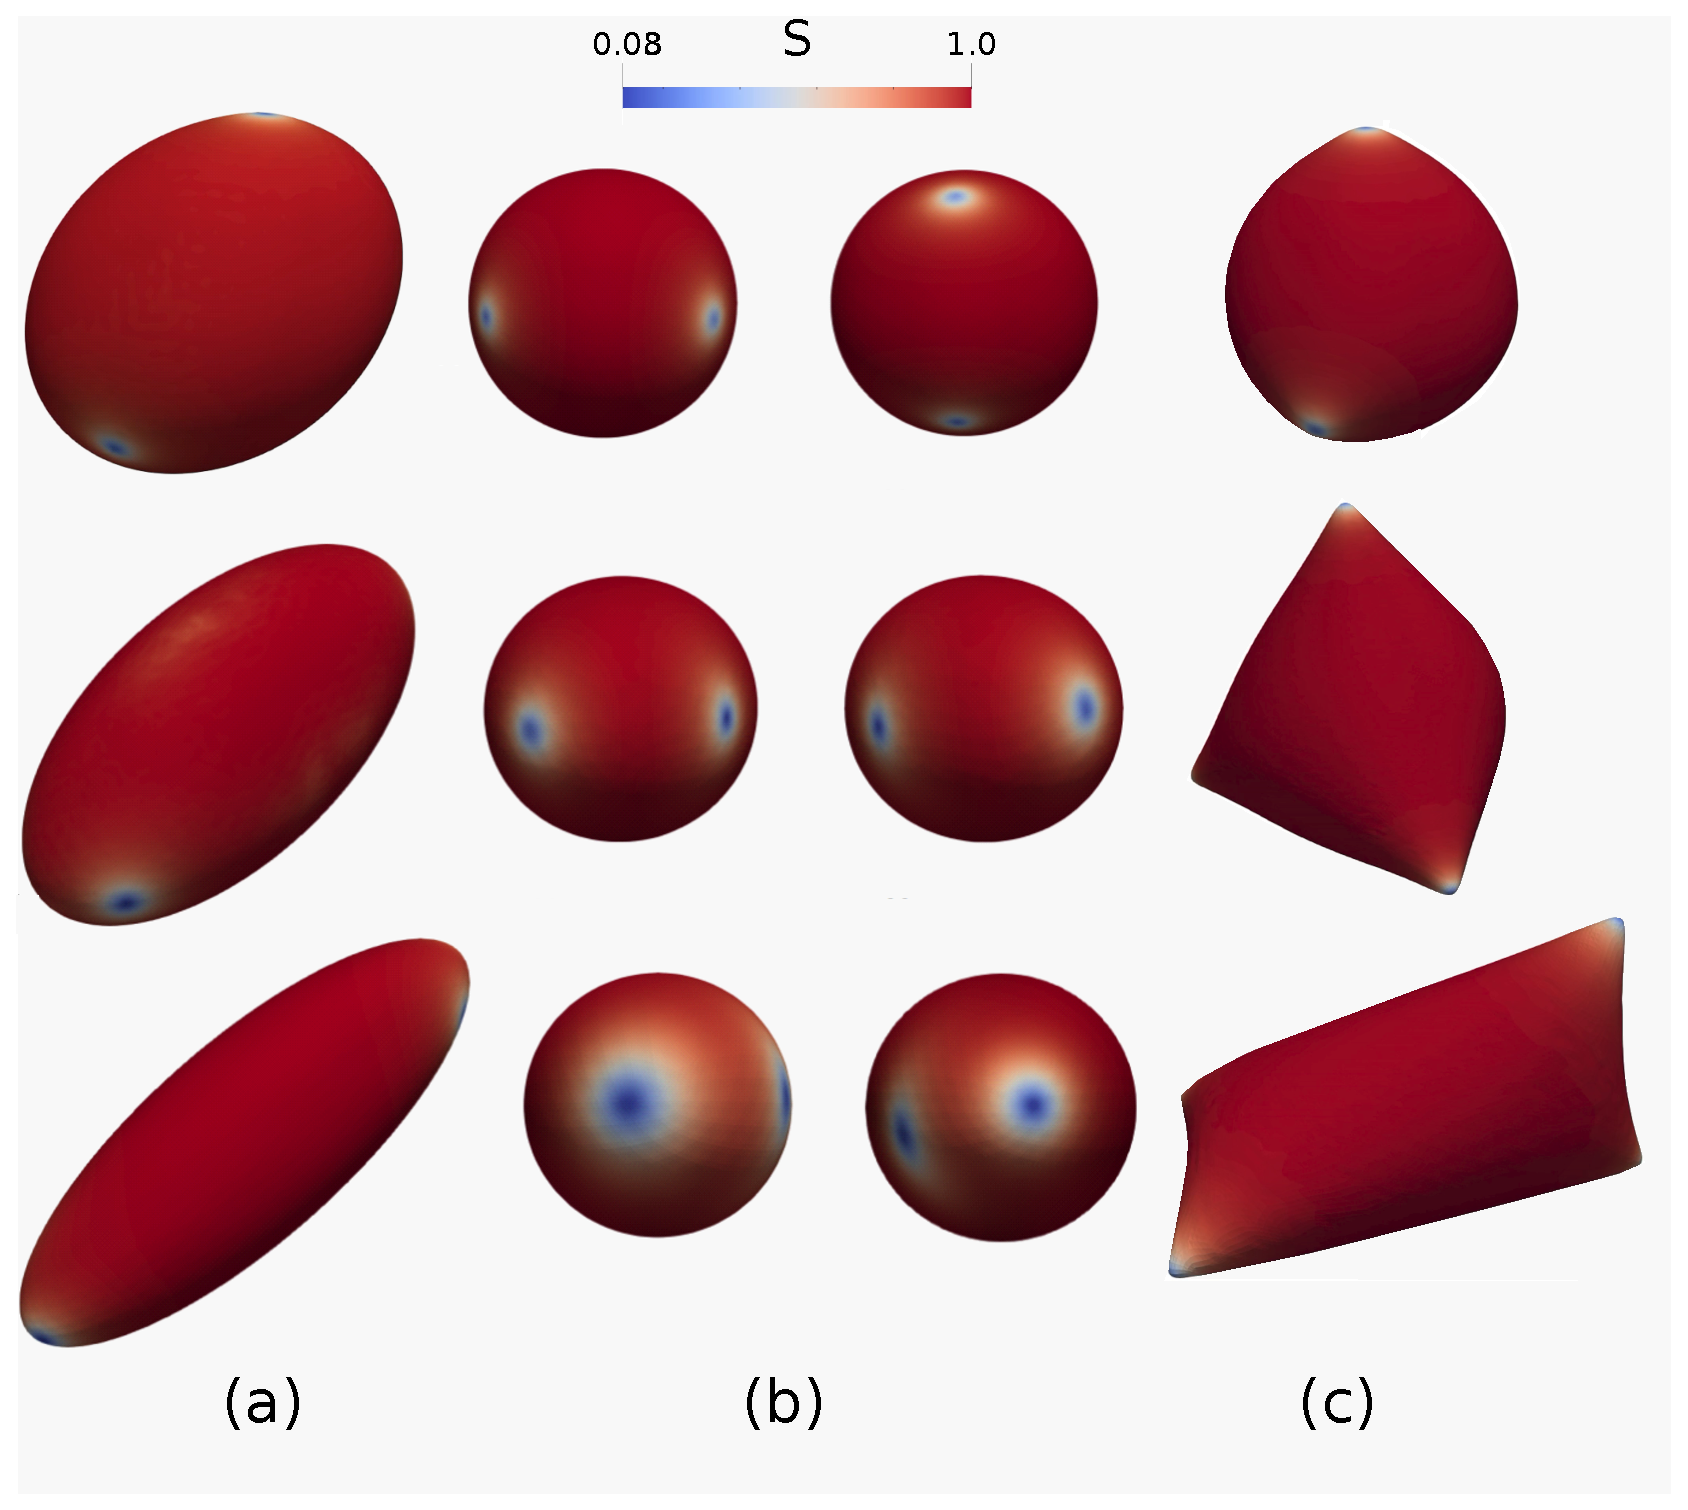
\includegraphics[width=1.\textwidth]{fig9.2.eps}
	\caption{ \textbf{Interplay between shape and nematic field}. (a-b) Different views of the configuration of defects on an initially ellipsoidal surface at short times $\propto \eta_{\rm rot }/|a|$. At these times, shape has not evolved and nematic order is nearly at equilibrium. (a) shows a 3D  perspective whereas (b) show front and back views. (c) Steady state at long times ($\gg \eta/|a|$) once both shape and nematic field have relaxed.  }
	\label{fig9.1}
\end{figure} 
  
 
 \subsection{Dynamics of an active nematic vesicle }
 
 We next examine the interplay between shape and nematic order for an active vesicle, which develops a transient limit cycle with moving defects, shape changes and interfacial flows. Now, nematic and shape relaxations happen at comparable time-scales, $\eta /\eta_{\rm rot} = 1$.

  First, we deflate a spherical passive vesicle by $10\%$ of the original volume, resulting in the formation of an excess membrane due to the inextensibility constraint. We then allow the system to relax, resulting after an interesting transient in a tetrahedral configuration with four $+1/2$ pointy defects, Fig.~\ref{fig9.2}(a-e). We next turn non activity, $\lambda_{\rm aniso}\ne 0$. If activity is small, it only results in a slight change of shape and nematic field. Above a threshold, it leads to a persistent motion of defects and shape changes. During these dynamics, the system  periodically leaves a low-energy tetrahedral state to evolve towards a different symmetry-related tetrahedral state passing through a high-energy state with a planar defect configuration, Fig.~\ref{fig9.2}(f-j) and \href{https://github.com/waleedmirzaPhD/movies_thesis.git}{Movie~$8.5,8.6$}. These results are in agreement with experimental observations on active nematic vesicles \cite{keber2014}.

  
 
 \begin{figure}
 	\centering
 	\hspace*{-0.5cm}\includegraphics[width=1.\textwidth]{fig9.1.pdf}
 	\caption{ \textbf{Effect of activity on the dynamics of defects and shape changes}. (a-e) A passive liquid crystal vesicle is deflated to generate excess area. Afterwards, the nematic field and shape are  allowed to relax, leading to four pointy  $+1/2$ defects in a tetrahedral arrangement. (f-j) The presence of finite activity generates active flows around the defects, which periodically deforms the vesicle oscillating between low-energy tetrahedral states and high-energy planar states.  }
 	\label{fig9.2}
 \end{figure} 
